%\subsection{Tapered waveguide due to taper length}
%tapered_length
The value of the divergence angle is also an important property of the tapered waveguide to determine the coupling ability. In order to simplify the modeling process the variation of taper length, instead of divergence angle, will be performed in the following coupling simulations. \\

As before the waveguide is placed at the distance of $4\mu$m from the TLF. The taper width is kept  as a constant of $d_{1}=2\mu$m and the taper length is changed from $L_{taper}=2\mu$m to $ L_{taper}=5.5\mu$m in following simulations.\\
  
\begin{figure}[!ht]
\centering
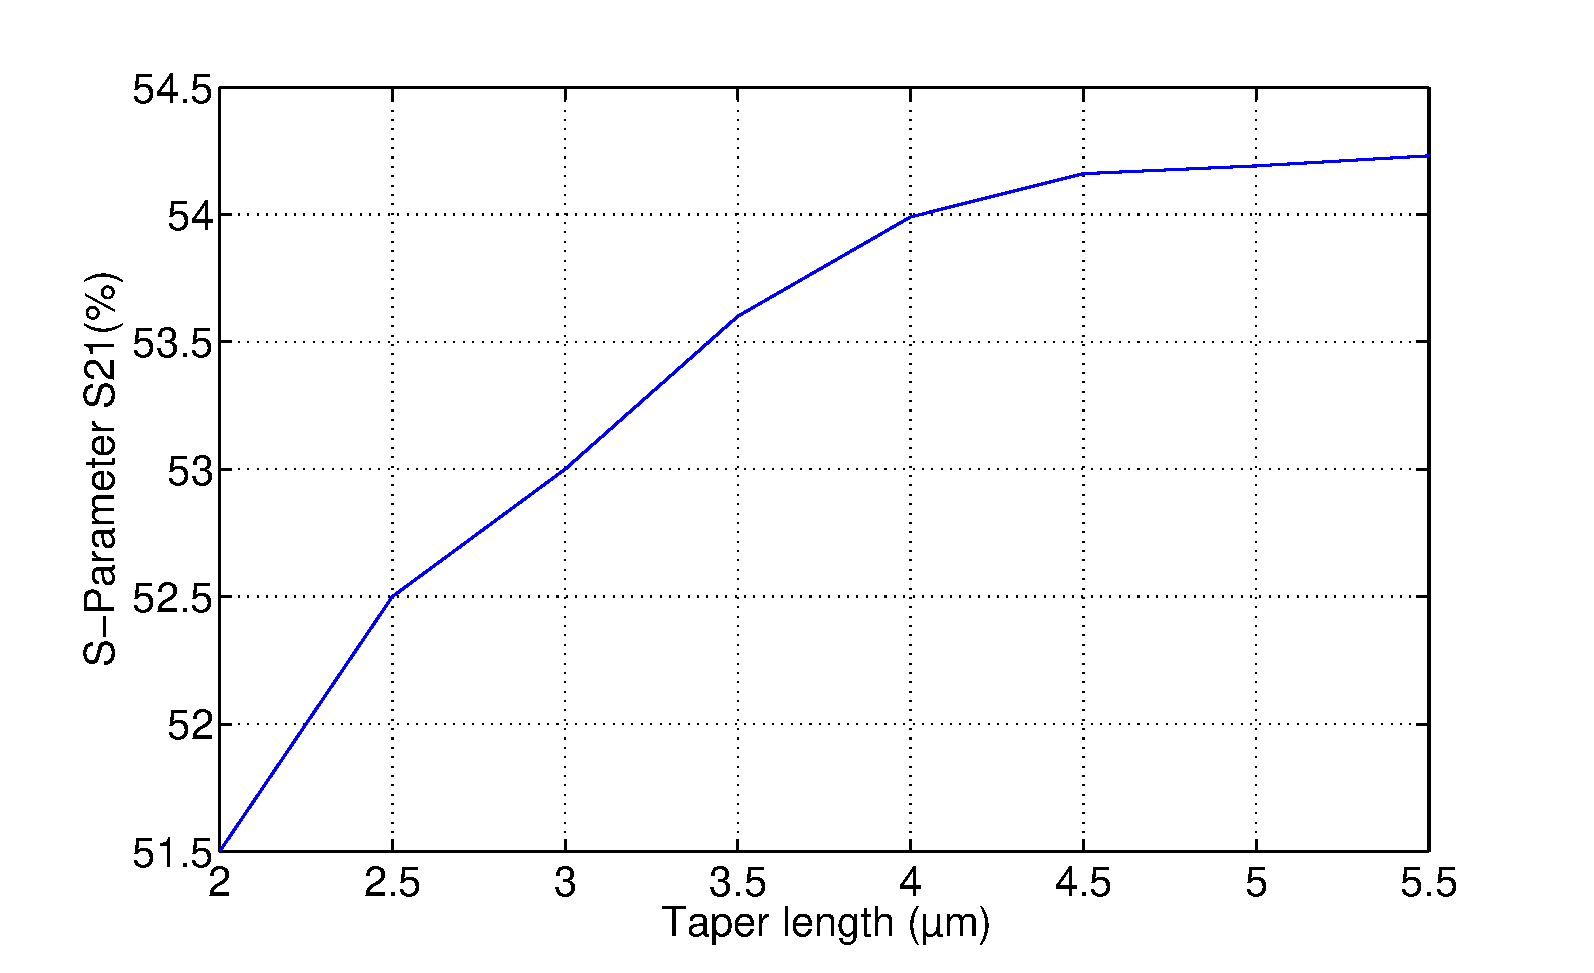
\includegraphics[width=0.7\textwidth]{bilder/tapered_waveguide_dxx}
\caption{Coupling efficiency between TLF and tapered waveguide due to taper length and taper width $= 2\mu$m.}
\label{fig:tapered_waveguide_dxx}
\end{figure}
Fig. \ref{fig:tapered_waveguide_dxx} exhibits the coupling behavior for varying the taper length from $2\mu$m to $5.5\mu$m. The coupling efficiency starts with the value of $51.5\%$ and is rising monotonously with the taper length increasing. After taper length $4.5\mu$m of the coupling efficiency rise more and more gently, close to a constant $54.2\%$. 
Therefore, for an efficient coupling the optimal divergence angle of the taper in this arrangement is less than:
\begin{equation}
\theta=\arctan\frac{d_{1}-d_{0}}{L_{taper}}=\arctan\frac{2-1}{5.5}=10.3^{o}
\label{eq:divergence_angle}
\end{equation}
The reason of this trend is explained by mode conversion for light propagating in tapers. In \cite{integrated_optics,mode_conversion_optical_waveguide} mode conversion in taper is analyzed through the local normal mode theory. The taper is divided into small steps as Fig. \ref{fig: discontinue_taper}. Each step is regarded approximately as an unvaried guide. Supposing the incident mode $i$ propagates from $m$th step to $m+1$th step, part of the power is converted to that of the high-order mode $j$ in step $m+1$. At the end of the taper more modes are converted and more power of incident mode is converted. But the mode conversion in a linear taper can be minimize by controlling the aspect ratio $L_{taper}/d_{1}$ . A high aspect ratio makes the transition more gradual in the taper, thus leading to limited mode conversion. Yip's result in \cite{mode_conversion_optical_waveguide} showed that power converted from incident mode to high-order modes can be controlled under $5\%$ for an aspect ratio over $100$.\\

\begin{figure}[!ht]
\centering
\includegraphics[width=0.7\textwidth]{bilder/discontinue_taper}
\caption{Taper is divided into discontinued steps.}
\label{fig: discontinue_taper}
\end{figure}

From previous discussions about taper structure following advices can be given for design of the efficient tapered waveguide:
\begin{itemize}
\item The taper width should expand enough wide to adapt the spot size of  incident light. 
\item The aspect ratio $L_{taper}/d_{1}$ should be big enough to minimize mode conversion.
\end{itemize} 
